\section{Lessons Learned}
\label{sec:lessons}

\FIXME{What are the lessons we have learned?}

\FIXME{Assignments with a duration of only one week.}

\FIXME{Extra credit experiment and results. Figure~\ref{fig:scores}.}

Based on commentary that posits the benefits of analysis problems
in the context of design courses, we were concerned that the present
course doesn't have sufficient analysis content (i.e., the bulk of
studio questions and assignment questions are design questions rather
than analysis questions).

To test this theory, we generated an additional set of analysis problems,
designed to be helpful in preparing students for the third exam, and
made them available to students one week prior to the exam.  To provide
an incentive for the students to attempt them, students were told that
there would be a small amount of extra credit for those that did well.

We then compared scores for the two groups of students, those who did
attempt the extra credit exercise and those who did not.  The results
of this comparison are shown in Figure~\ref{fig:scores}.
There clearly is a correlation between overall course grade and
whether or not a student attempted the extra exercise.
Those who attemped the extra exercise scored over 4\% higher overall
(the scores presented exclude the extra credit provided from the
exercise).  This is statistically significant at $p = 0.02$ (non-paired data).

\begin{figure}[ht]
\centering
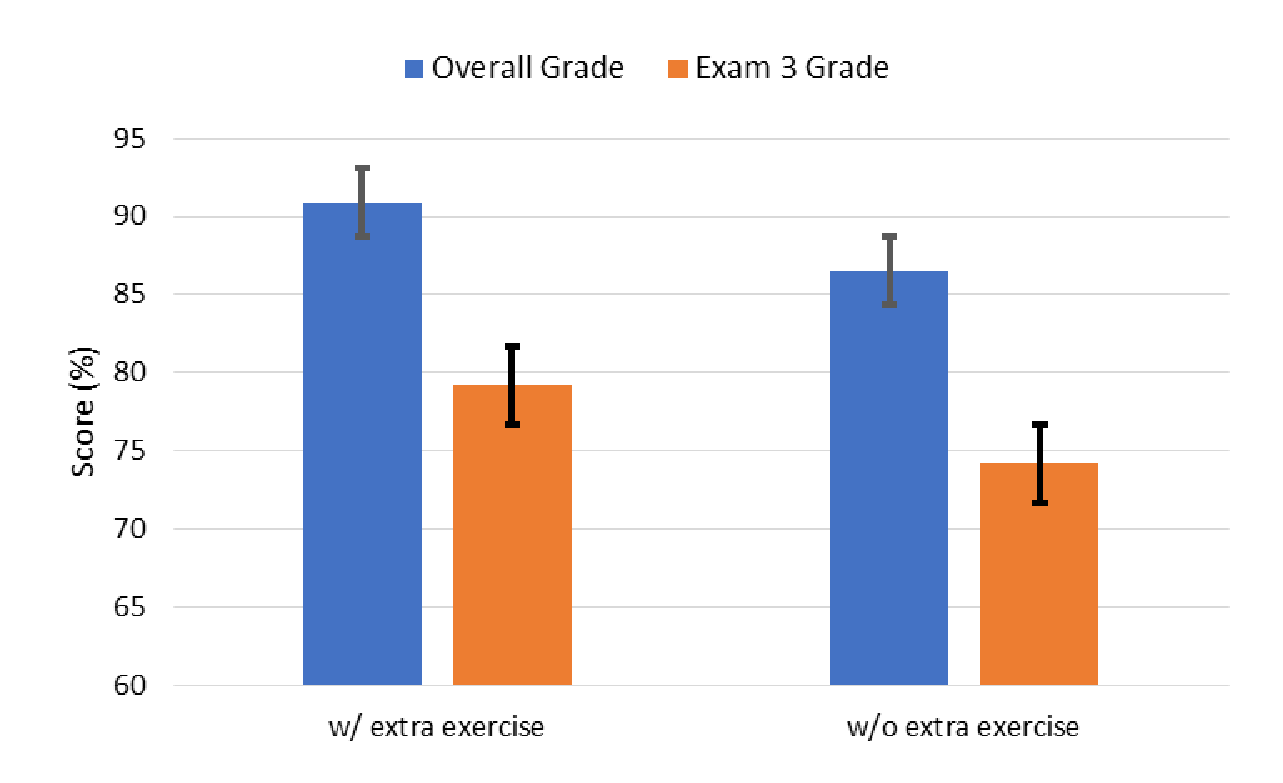
\includegraphics[width=\columnwidth]{scores}
\caption{Relationship between overall scores and exam~3 scores
with and without the extra exercise. The bars indicate mean score and
the whiskers indicate standard error.}
\label{fig:scores}
\end{figure}

When we examine the scores on exam~3, however, the story is different.
While the mean score differential is similar (at 5\% in this case), the
variability in scores is wide enough that this result is not
statistically significant ($p = 0.11$, non-paired data), so we cannot
rule out the null hypothesis that the difference in the means is
due to chance.

Our current opinion is that the correlation seen in the overall scores
is nothing as specific as a single exercise, but is more likely due to the
fact that better students (more likely to achieve a higher score prior
to the availability of an optional exercise) are also more likely than
their peers to take advantage of an optional exercise, especially when
it provides extra credit.

Going forward, we are still interested in whether or not additional
analysis problems can help students learn the material better, and will
likely pursue it by altering the mix of analysis vs.~design problems
within the studio exercises.

``More structure and organization, use more difficult examples when
teaching the material since the assignments were a lot harder than
the given examples.''

``It needs more organization.'' We didn't do as good a job as we should have
in communicating due dates, etc. A number of the specifics on the calendar
were filled out (made available to the students) as the semester proceeded.
In retrospect, this was a mistake, as a number of things didn't make it on
to the calendar early enough for everyone to see them.
